\section{Portfolio: The Andolian Protectorate}
Ships overview for all groups (Work In Progress): \href{http://vegastrike.sourceforge.net/wiki/Artstyle\_guide:Overview\_Guide}{Ship Overview} \\
Art-style Guide (Work In Progress): \href{http://vegastrike.sourceforge.net/wiki/Artstyle\_guide:Andolian\_Protectorate}{Artstyle Guide} \\
Species overviews: \href{http://vegastrike.sourceforge.net/wiki/Species:Humanity}{Species:Humanity} \\
 \href{http://vegastrike.sourceforge.net/wiki/Species:Klk\'k}{Species:Klk'k} \\
 \href{http://vegastrike.sourceforge.net/wiki/Species:Purth}{Species:Klk'k} \\

\subsection{Origin}
\begin{itemize}
\item Gravity: 

\item Atmosphere: 

\item Primary liquid bodies: 

\item Average temperature of homeworld (pre-industrialization):

\item Sun: 

\item Primary challenges (pre-industrialization): 
\end{itemize}

%ORIGIN COMMENTS GO HERE

\subsubsection{Habitat}

\subsection{Physical}
\begin{itemize}
\item Dimensions: 

\item Mass: 

\item Skeletal system: 

\item Major divisions: 

\item Senses: 

\item Visual acuity: 

\item Chemosense: 

\item Locomotion: 

\item Manipulators: 

\item Textural appearance: 
\end{itemize}

%PHYSICAL COMMENTS GO HERE

\subsection{Mental}


\subsection{Technological}
\begin{itemize}
\item Tech: 


\item Weapons:

\item Tactics:
\begin{itemize}
\item    Small groups: 
\item    Large groups/Fleets: 
\end{itemize}


\item Installations:


\end{itemize}

\subsection{Culture}

\subsubsection{Factions and Organizational Groups}
Listed below are noteworthy Aeran sub-factions and organizational groups: 
\begin{itemize}
\item FACTIONS GO HERE
\end{itemize}

\subsubsection{Religion}

\subsubsection{Cultural Aesthetics}

\subsection{Writing, numbers, and insignia}

\subsection{Faction: PRIMARY FACTION}

%Faction data 
%Aera 
%Species 	Aera 
%Homeworld (Origin) 	Aeneth 
%Capital 	Aeneth 


\subsubsection{A Brief History of the PRIMARY FACTION}


\subsubsection{Development}

\subsubsection{Culture}

\subsubsection{Organization}

\subsection{Faction: OTHER FACTIONS}

%Faction data 
%Merchant Marines 
%Species 	Aera 
%Homeworld (Origin) 	Aeneth 
%Capital 	Aeneth 


\subsection{Vessels Style}

\subsubsection{Style Overview}
\begin{itemize}

\item Primary distinguishing color ranges: 

\item Common accent colors:

\item Primary lighting color:

\item Frequently visible: 

\item Rarely visible:

\item Seen inside, but not out: 

\item Moving parts(non-turret): 

\item Capital vs. light craft: 

\end{itemize}

\subsubsection{Surface features of large vessels}

\subsubsection{Small things found on the hull of a large  vessel}
\begin{itemize}
\item Service/Maintenance hatches
\end{itemize}
{\it Somewhat larger things found on the hull of a large Aeran vessel:}
\begin{itemize}
\item Escape pod launcher ports
\end{itemize}
{\it Yet larger things ... :}
\begin{itemize}
\item Pinnace/lander launch bay (non-carrier vessels)
\end{itemize}

\subsection{Listing of vessels}

Existing concept art is not particularly canonical. Please redesign.

\subsubsection{Nietzsche}

Visual description: 
The basic shape of the main hull is roughly cylindrical. The thickness of the body does not vary overmuch, though it does vary, except at the front and rear. At the rear, it tapers abruptly for a very short time, then curves in on itself, creating a caldera, or bowl-like depression into the rear of the vessel. The main engine exhausts are in this inset area. On the tapered part of the ring around the engine bowl are four point-defense turrets, one top, bottom, and to each side. Coming out from the main hull are four projections, one pair on top and bottom, not too much after the engine area, and one pair on the sides, forward of the top and bottom pair, but overlapping somewhat in that they begin before the other pair ends. These projections are quite thick, and shaped something like a compromise between a circle and an equilateral triangle. Imagining them as triangles one would say that they were aligned such that the top and bottom pair pointed forwards, and the two side projections pointed rearwards. The projections extend out about the radius of the main body, whereupon they are capped by a thick, slightly wider plate, much as one would imagine a toadstool, shitake, or portabello would appear if the stalk were almost as thick as the head, and the head flat on the top and rounded on the bottom and edge. Just below the cap, embedded in the projections, are large engine thrusters. The engine thrusters in the top/bottom pair are larger than those in the side pair. On top of the cap, at each of the "corners" is a largish turret, though not a massive one, somewhat tilted down from the flat plane of the top of the cap such that its gun can depress below level. Each such turret contains a single gun. Forward of the side projections somewhat, the cylindrical main body differentiates. The top portion becomes a bundle of six tubes (for launching anti-capital missiles) around a larger central projection, two above, two below, and one to each side in slightly svertically squashed hexagonal fashion. The tubes are not actually touching each other, and the area in between them is filled in solid as is the area between the tubes and the central projection. Beneath this bundle of tubes is a hangar/docking bay. The combination of the docking bay and the collection of tubes are slightly slimmer than the main body of the ship. The tubes extend slightly beyond the end of the hangar. The central tube area terminates in an inset sensor array and two small turrets, one to each side. The missile launcher tubes terminate as one would expect them to, flush with the base of the turrets on the central projection. There is a tractor beam turret on both sides of the hangar, and a disabling turret on the bottom lip of the hangar. 

There are various PD and anti-fighter turrets, but their position isn't as important at this level of description, save to say that I see 3 anti-fighter turrets on the sides of each projection to discourage loitering beneath the guns, and that PD coverage must be excellent :) 

FIXME To describe a bit more... 

The open face of the docking bay is in the forward direction, and though, from the outside, it is clearly much deeper, the initial open area is somewhat shallow as it terminates in a large armored door that protects the inner docking bay. 

Looking at the Nietzsche from dead ahead of the vessel, one might imagine the missile launcher tubes as the hideously deformed descendants of magazine from a six-shooter revolver. Relative to the crisp radial symmetry of the six-shooter, the tubes are stretched further apart horizontally, maintaining vertical and horizontal symmetry, but not radial. Likewise, the apertures where the missiles exit are vastly smaller by comparison to the size of the tubes themselves than in a revolver. Most notably of course, these tubes do not at all revolve, nor move at all. So they really do not look all that much like a revolver magazine; perhaps the image of a revolver is only the quick shadow of a thought that comes from knowing that one is staring at six tubes, each of which holds death, and each of which has opened its dark mouth in your direction.... 

Materials/texture/greebles/etc. appearance: A purely military vessel, there are no vulnerable areas exposed unnecessarily. However, there are various sensor arrays, shield emitters, escape pod launchers, and maneuvering thrusters located on the hull, so it is not just a giant smooth armored mass. That being said, it IS a military vessel, and the dominant feature of its hull will still be the nearly seamless overlapping plates of multiple layers of armor. 

Approximate Sizes: length of main body - 1500 meters, including engines, hangar bay and launch tubes. radius of main body, 150 meters. length of projection caps ~ 450 meters 

\begin{figure}
\begin{center}
\makebox[\textwidth][c]{
    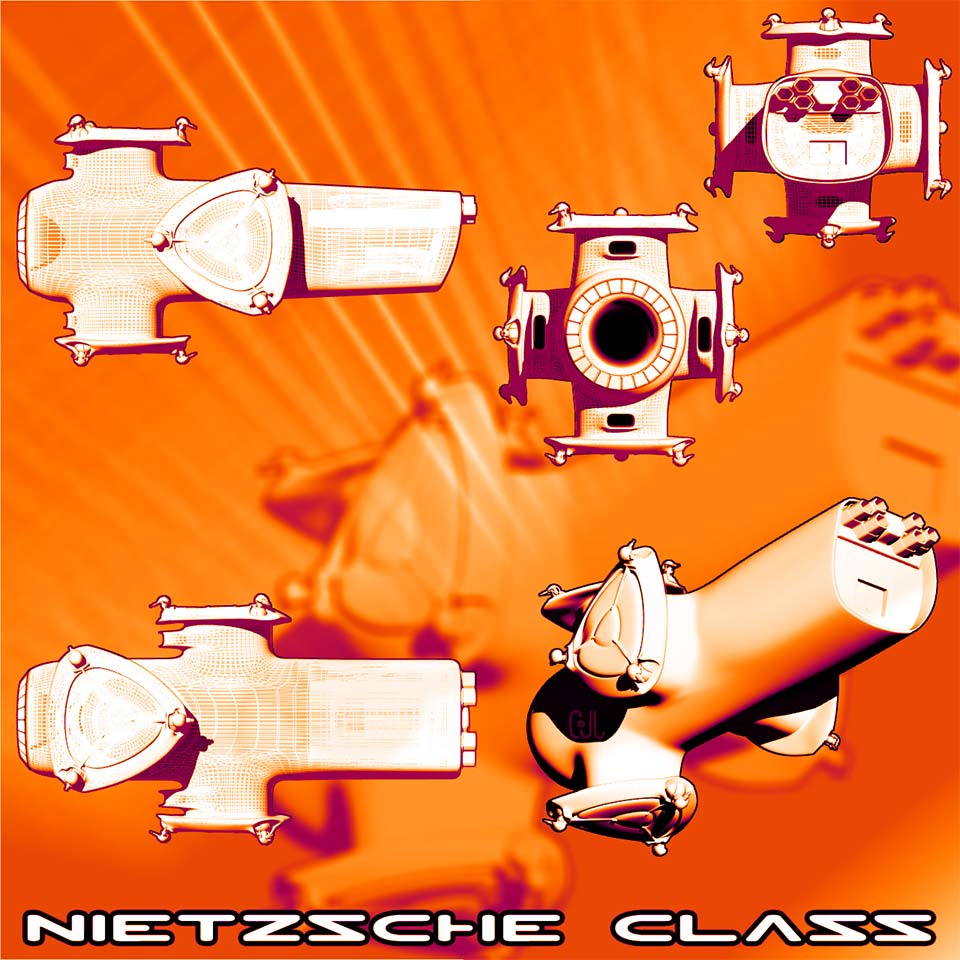
\includegraphics[width=\textwidth]{../images/vessels/NietzscheSchematics.jpg}
}
    \caption{A translated version of the above visual description for the Andolian Protectorate's Nietzsche capital vessel.}
    \label{fig:vessel-nietsche}
\end{center}
\end{figure}




% LocalWords:  Aerans Aeran Artstyle Aera Pinnace Acrotatus Agasicles Agesilaus
% LocalWords:  Agesipolis Agis Alcmenes Anaxander Wiki Anaxandridas Rlaan Areus
% LocalWords:  Anaxidamus Ariston Charillus Cleombrotus Cleomenes Demaratus Uln
% LocalWords:  Theopompus Dorissus Echestratus Eurycratides Eurypon Leons Bzbr
% LocalWords:  Nicander Pausanias Pleistarchus UnAeranned Pleistoanax Andolian
% LocalWords:  Spaceborn's MacGyver Polydectes Polydorus EVAs Procles Prytanis
% LocalWords:  Soos Teleclus terraforming Aenethforming Zeuxidamus homeworld
% LocalWords:  coreward chemoreception Klk'k Aeneth ecologies Shmrn
